\chapter{Chapter One}
\label{cha:one}

Lorem ipsum dolor sit amet, consetetur sadipscing elitr, sed diam nonumy eirmod tempor invidunt ut labore et dolore magna aliquyam erat, sed diam voluptua. At vero eos et accusam et justo duo dolores et ea rebum. Stet clita kasd gubergren, no sea takimata sanctus est Lorem ipsum dolor sit amet. Lorem ipsum dolor sit amet, consetetur sadipscing elitr, sed diam nonumy eirmod tempor invidunt ut labore et dolore magna aliquyam erat, sed diam voluptua. At vero eos et accusam et justo duo dolores et ea rebum. Stet clita kasd gubergren, no sea takimata sanctus est Lorem ipsum dolor sit amet.


Therefore, this chapter presents research that structures existing research and conceptual knowledge to understand the function of \ac{bpm} (\Cref{sec:one_a}; \Citen{paper_a}). 


\section{Part One A}
\label{sec:one_a}

Lorem ipsum dolor sit amet, consetetur sadipscing elitr, sed diam nonumy eirmod tempor invidunt ut labore et dolore magna aliquyam erat, sed diam voluptua. At vero eos et accusam et justo duo dolores et ea rebum. Stet clita kasd gubergren, no sea takimata sanctus est Lorem ipsum dolor sit amet. Lorem ipsum dolor sit amet, consetetur sadipscing elitr, sed diam nonumy eirmod tempor invidunt ut labore et dolore magna aliquyam erat, sed diam voluptua. At vero eos et accusam et justo duo dolores et ea rebum. Stet clita kasd gubergren, no sea takimata sanctus est Lorem ipsum dolor sit amet.

\citen{paper_a} is a paper that contains a picture of a giraffe, as can be seen in \cref{m:fig:giraffe}.

\begin{figure}
    \centering
    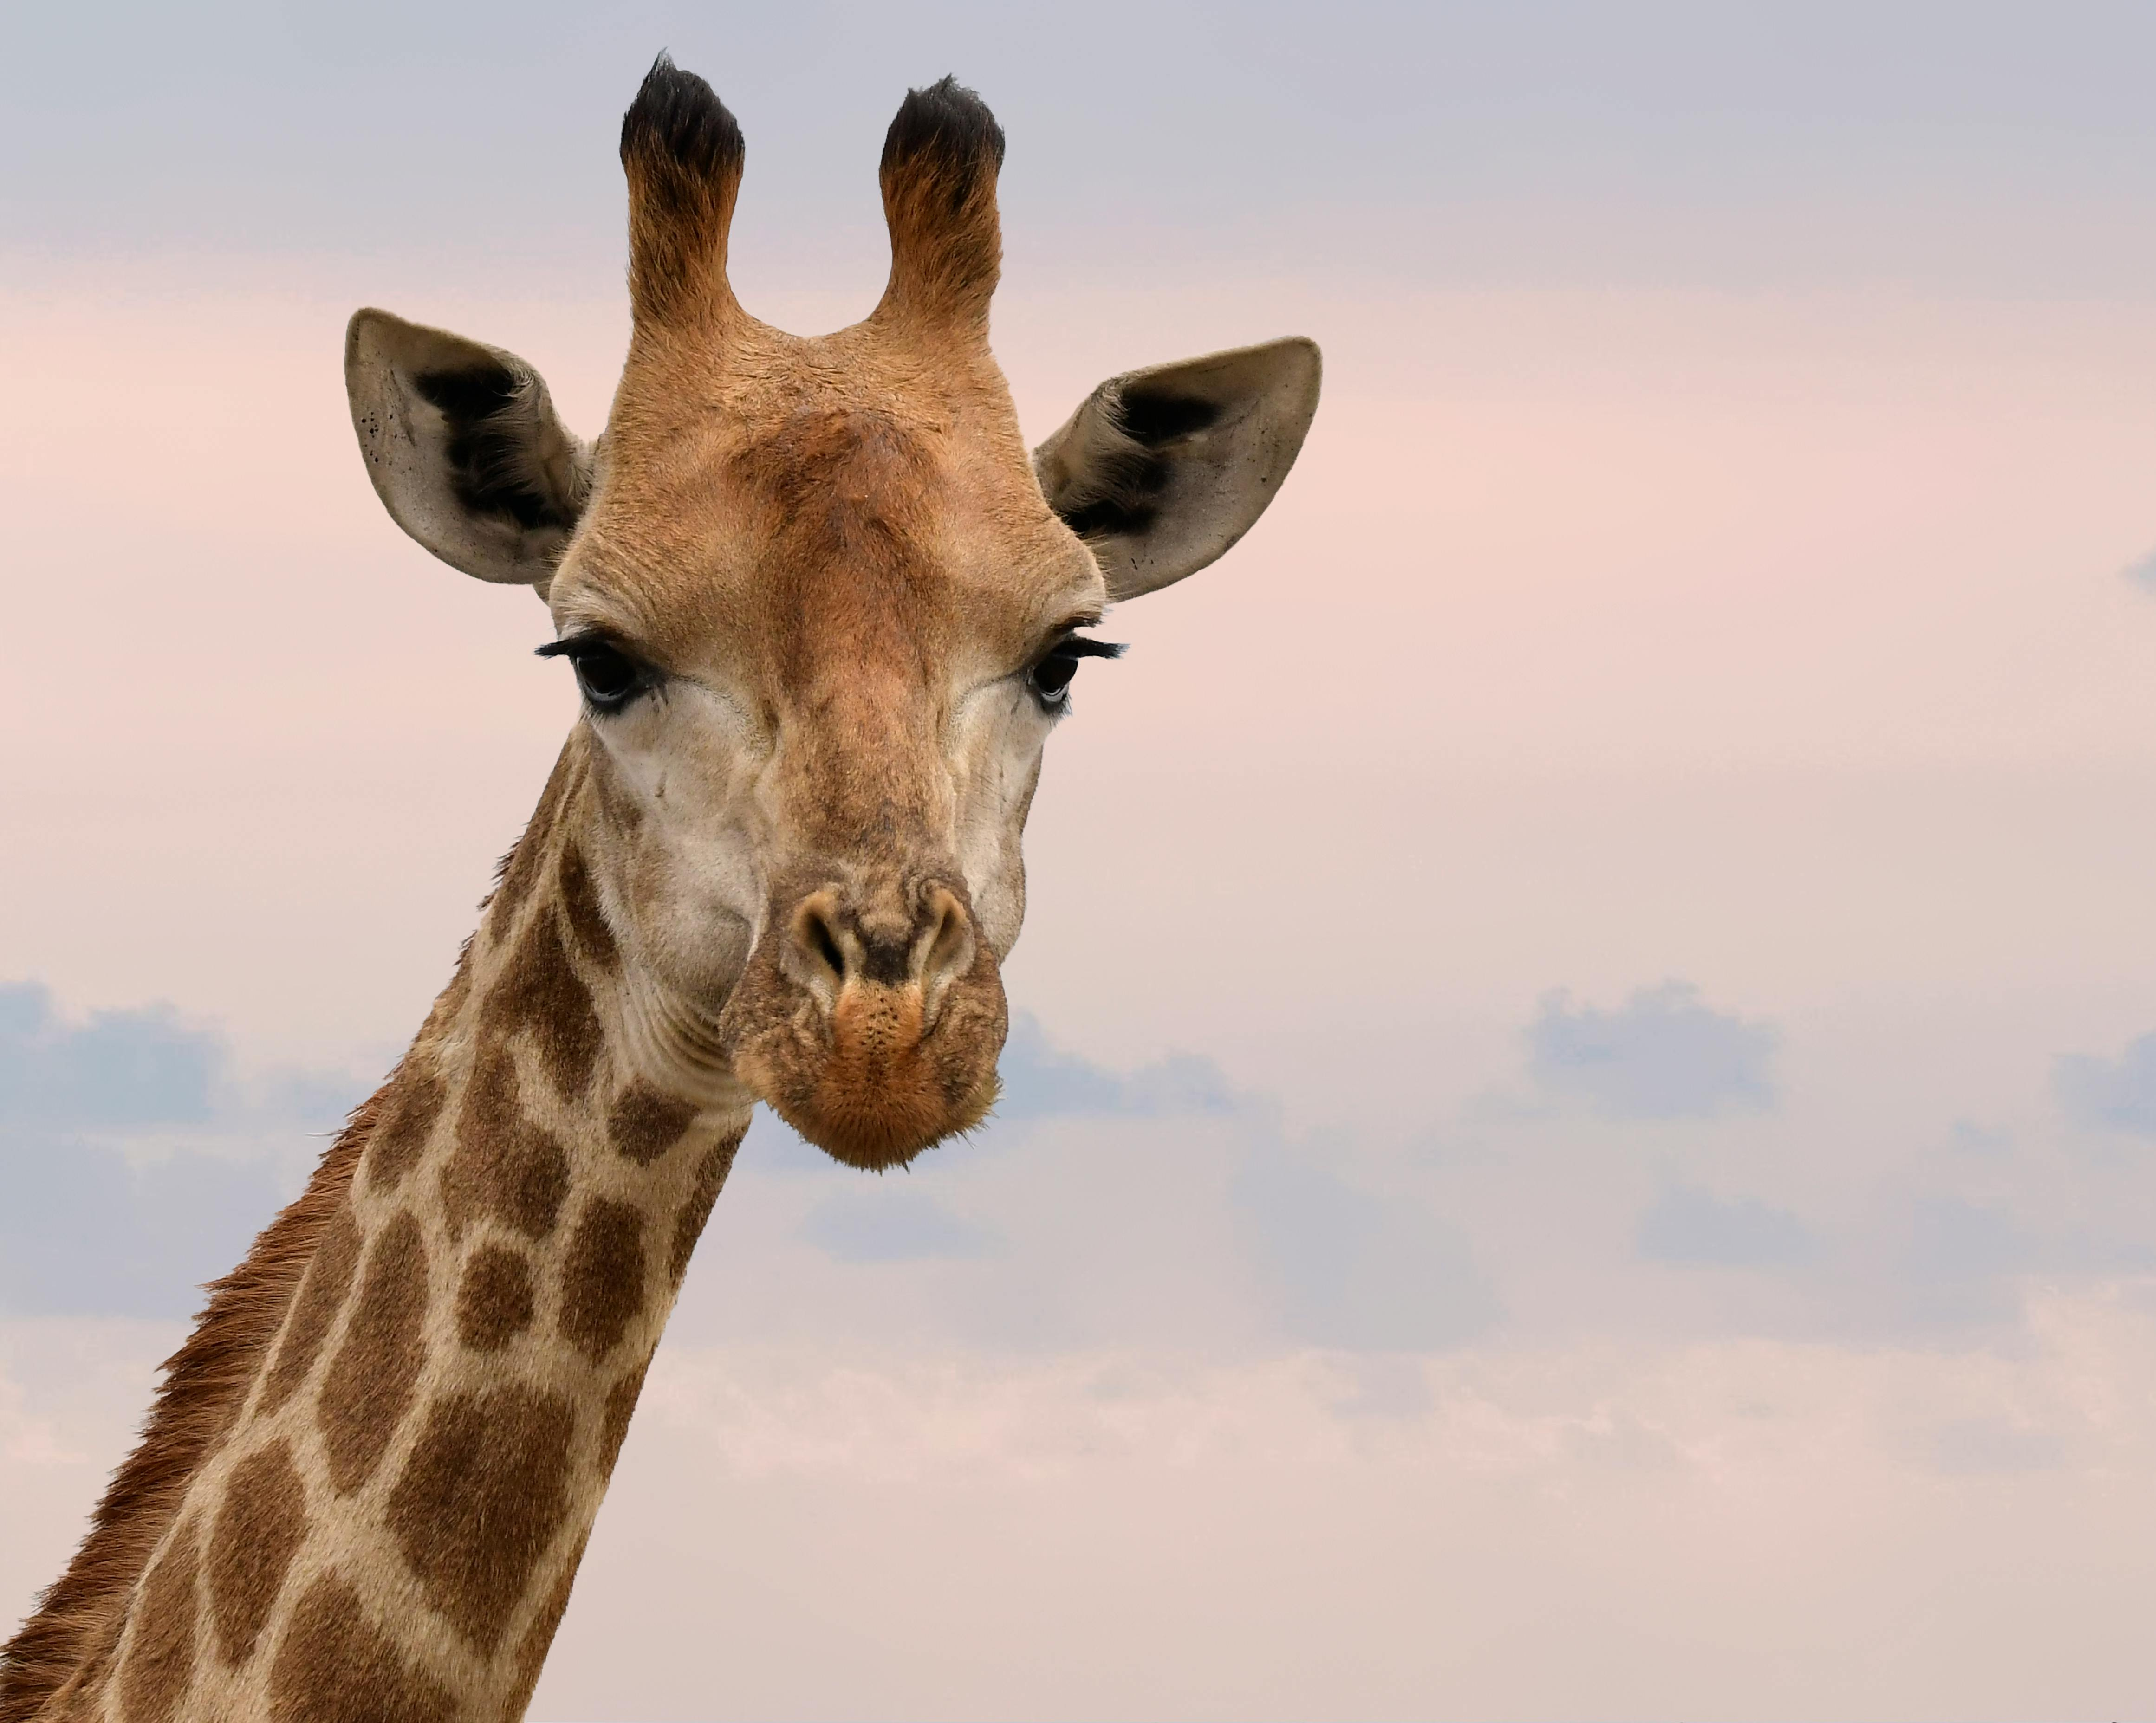
\includegraphics[width=0.5\linewidth]{figures/paper_a/pexels-frans-van-heerden-201846-802112.jpg}
    \caption{Giraffe, Frans van Heerden: https://www.pexels.com/de-de/foto/nahaufnahme-fotografie-der-giraffe-802112/ }
    \label{m:fig:giraffe}
\end{figure}